\chapter{Wireless and Mobile Networks: 802.11 and Beyond}\label{ch:wireless}
\begin{quote}
\emph{``Wires tell you where the network is; wireless tells you where it could fail.''} --- From fighting fading and hidden terminals to handing off a phone call at 300\,km/h, this chapter makes wireless concrete: why CSMA/CD does not work in air, how Wi-Fi dodges collisions without detecting them, and how cellular keeps you connected while moving.
\end{quote}

\noindent\fbox{\parbox{\dimexpr\linewidth-2\fboxsep-2\fboxrule}{%
\textbf{From zero: we build here, no prior wireless knowledge needed.} We start from intuition---shouting across a noisy room---then formalise: SNR, path loss, and medium access. Every 802.11 and cellular idea is introduced as picture $\to$ words $\to$ definition, then tied to the IP stack you already know.}}%
\vspace{0.4em}

\section*{Learning Outcomes}
After this chapter you will be able to:
\begin{enumerate}[label=(L\arabic*)]
    \item explain why wireless links differ from wired: fading, hidden terminals, and bit errors;
    \item describe 802.11 architecture (BSS, ESS, AP, channels) and why association matters;
    \item analyse CSMA/CA with DIFS/SIFS, backoff, RTS/CTS and NAV;
    \item sketch the 802.11 frame and explain rate adaptation and mobility handoff;
    \item outline cellular evolution (2G/3G/4G/5G) and Mobile IP triangle routing.
\end{enumerate}

% ============================================================
\section{Why Wireless Is Hard: Intuition First}\label{sec:wireless-hard}
Imagine two people shouting across a courtyard with a wall between them. They cannot hear if the other is already shouting (no collision detection), the wall attenuates sound (fading), and a third person near each listener hears differently (hidden terminal). Wireless is exactly this: a shared, noisy, distance-dependent broadcast medium.

Formally, received power follows path loss $P_r \propto P_t / d^{\alpha}$ with $\alpha\in[2,4]$, plus shadowing and multipath fading that makes $P_r$ vary on millisecond scales. Signal-to-noise ratio $\mathrm{SNR}=P_r/N_0$ sets bit-error rate (BER); higher SNR $\to$ lower BER $\to$ more bits per symbol (e.g., BPSK $\to$ 64-QAM). A \emph{hidden terminal} is $A$--$B$--$C$ where $A$ and $C$ cannot hear each other but both can reach $B$; an \emph{exposed terminal} is $B\to A$ blocking $C\to D$ though the two transfers would not collide.

\begin{figure}[h]
\centering
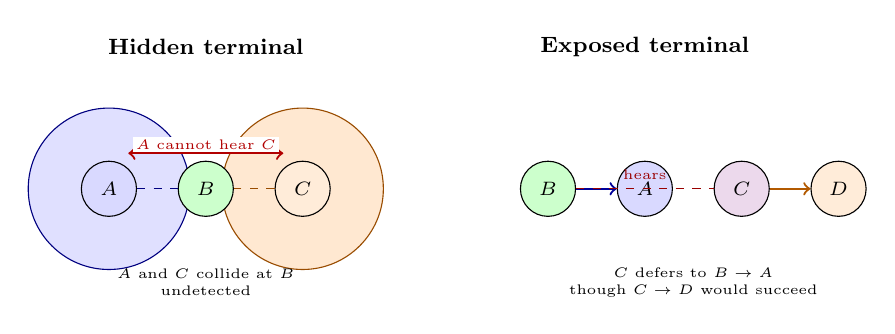
\begin{tikzpicture}[scale=0.82,every node/.style={font=\scriptsize}]
% Hidden terminal
\begin{scope}
\node[font=\footnotesize\bfseries] at (1.5,2.2) {Hidden terminal};
\draw[fill=blue!12,draw=blue!50!black] (0,0) circle (1.25);
\draw[fill=orange!18,draw=orange!60!black] (3,0) circle (1.25);
\node[draw,circle,fill=green!20,minimum size=7mm] (B) at (1.5,0) {$B$};
\node[draw,circle,fill=blue!15,minimum size=7mm] (A) at (0,0) {$A$};
\node[draw,circle,fill=orange!15,minimum size=7mm] (C) at (3,0) {$C$};
\draw[dashed,blue!50!black] (A) -- (B);
\draw[dashed,orange!60!black] (C) -- (B);
\draw[<->,red!70!black,thick] (0.3,0.55) -- (2.7,0.55) node[midway,above,font=\tiny,fill=white,inner sep=1pt] {$A$ cannot hear $C$};
\node[font=\tiny,align=center] at (1.5,-1.45) {$A$ and $C$ collide at $B$\\undetected};
\end{scope}
% Exposed terminal
\begin{scope}[xshift=6.8cm]
\node[font=\footnotesize\bfseries] at (1.5,2.2) {Exposed terminal};
\node[draw,circle,fill=green!20,minimum size=7mm] (B2) at (0,0) {$B$};
\node[draw,circle,fill=blue!15,minimum size=7mm] (A2) at (1.5,0) {$A$};
\node[draw,circle,fill=violet!15,minimum size=7mm] (C2) at (3,0) {$C$};
\node[draw,circle,fill=orange!15,minimum size=7mm] (D2) at (4.5,0) {$D$};
\draw[->,thick,blue!60!black] (B2) -- (A2);
\draw[->,thick,orange!70!black] (C2) -- (D2);
\draw[dashed,red!60!black] (B2) -- (C2) node[midway,above,font=\tiny] {hears};
\node[font=\tiny,align=center] at (2.25,-1.45) {$C$ defers to $B\to A$\\though $C\to D$ would succeed};
\end{scope}
\end{tikzpicture}
\caption{Left: hidden terminal --- $A$ and $C$ hidden from each other collide at $B$. Right: exposed terminal --- $C$ is needlessly blocked. Both motivate RTS/CTS and carrier sensing.}
\label{fig:hidden-exposed}
\end{figure}

Wired Ethernet can detect collisions while transmitting (CD) because the signal on the wire is observable. On wireless, a sender cannot listen while sending (its own power drowns others) and not all senders hear each other. So 802.11 avoids collisions rather than detecting them.

\section{802.11 Architecture: BSS, ESS, and Channels}\label{sec:802-arch}
The basic unit is the \emph{Basic Service Set (BSS)}: one Access Point (AP) plus its associated stations. In \emph{infrastructure} mode every frame goes through the AP, even $A\to B$ within the same BSS. An \emph{Extended Service Set (ESS)} links multiple BSSs via a distribution system (usually wired Ethernet), sharing one SSID. \emph{Ad hoc} (IBSS) has no AP; stations talk peer-to-peer.

Each BSS operates on a channel. At 2.4\,GHz there are 11 (US) overlapping channels; only 1, 6, 11 are non-overlapping (22\,MHz each). At 5\,GHz, 20/40/80\,MHz channels offer many non-overlapping options and higher rates. An AP chooses a channel to minimise interference; clients scan (active probe or passive beacon listen) then \emph{associate} via authentication and association frames. The AP maintains an association table mapping station MAC $\to$ BSS.

mobility within an ESS requires handoff: the station reassociates to a new AP; the distribution system updates forwarding. We revisit handoff formally in \S\ref{sec:mobility}.

\section{Medium Access: CSMA/CA in Depth}\label{sec:csma-ca}
Carrier Sense Multiple Access with Collision Avoidance is the heart of Wi-Fi. Rules:

\begin{enumerate}[itemsep=0.3em]
    \item Sense channel: if idle for DIFS (e.g., 50\,$\mu$s), transmit. If busy, defer and enter backoff.
    \item Backoff: pick uniform $k\in[0,\mathrm{CW}]$, wait $k\times$SlotTime while channel idle; freeze timer when busy; resume when idle for DIFS. CW starts at $\mathrm{CW}_{\min}$ (15) and doubles on collision up to $\mathrm{CW}_{\max}$ (1023).
    \item Receiver waits SIFS (10\,$\mu$s) then sends ACK. SIFS $<$ DIFS so ACK wins over new data.
    \item Optional RTS/CTS: sender sends short RTS, receiver replies CTS; both carry duration in NAV (network allocation vector) so neighbours that hear either frame defer, solving hidden terminals. Overhead makes RTS/CTS worthwhile only for large frames.
\end{enumerate}

\begin{figure}[h]
\centering
\resizebox{\linewidth}{!}{%
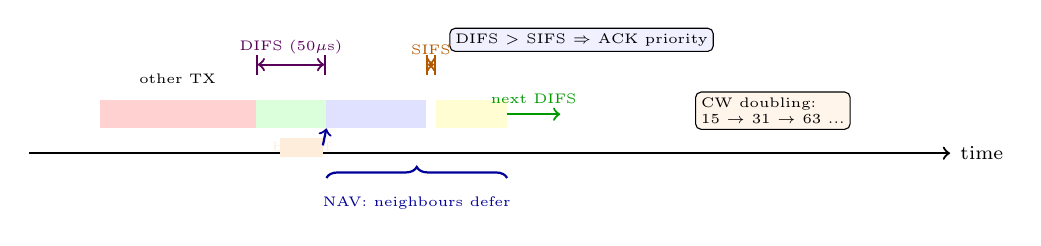
\begin{tikzpicture}[every node/.style={font=\scriptsize},scale=0.9]
% Timeline
\draw[thick,->] (0,0) -- (13,0) node[right] {time};
% Channel busy/idle bars
\fill[red!18] (1,0.35) rectangle (3.2,0.75) node[midway,font=\tiny] {busy};
\fill[green!14] (3.2,0.35) rectangle (4.2,0.75) node[midway,font=\tiny] {idle};
\fill[blue!12] (4.2,0.35) rectangle (5.6,0.75) node[midway,font=\tiny] {DATA};
\fill[yellow!18] (5.75,0.35) rectangle (6.75,0.75) node[midway,font=\tiny] {ACK};
\node[font=\tiny] at (2.1,1.05) {other TX};
% Marks
\draw[thick,|<->|,violet!70!black] (3.2,1.25) -- (4.2,1.25) node[midway,above,font=\tiny] {DIFS (50$\mu$s)};
\draw[thick,|<->|,orange!70!black] (5.6,1.25) -- (5.75,1.25) node[midway,above,font=\tiny] {SIFS};
% Backoff
\fill[orange!14] (3.55, -0.05) rectangle (4.15,0.22) node[midway,font=\tiny] {backoff};
\draw[->,thick,blue!60!black] (4.15,0.11) -- (4.2,0.35);
% Stations
\node[font=\tiny,align=left,fill=blue!6,draw,rounded corners=2pt,inner sep=2pt] at (7.8,1.6) {DIFS $>$ SIFS $\Rightarrow$ ACK priority};
\node[font=\tiny,align=left,fill=orange!8,draw,rounded corners=2pt,inner sep=2pt] at (10.5,0.6) {CW doubling:\\15 $\to$ 31 $\to$ 63 ...};
\draw[->,thick,green!60!black] (6.75,0.55) -- (7.5,0.55) node[midway,above,font=\tiny] {next DIFS};
% NAV
\draw[thick,decorate,decoration={brace,amplitude=4pt},blue!60!black] (4.2,-0.35) -- (6.75,-0.35) node[midway,below,yshift=-3pt,font=\tiny] {NAV: neighbours defer};
\end{tikzpicture}}%
\caption{CSMA/CA timing: wait DIFS, count down backoff only while idle, transmit, wait SIFS for ACK. NAV from RTS/CTS reserves the channel at neighbours.}
\label{fig:csma-ca-timing}
\end{figure}

\begin{lstlisting}[language=Python]
import random
CW_min, CW_max, SLOT = 15, 1023, 9  # slots, microsec
def csma_ca_transmit(channel_busy_fn, max_retries=6):
    CW = CW_min
    for attempt in range(max_retries+1):
        # 1. wait for DIFS idle (simplified: poll)
        while channel_busy_fn(): pass
        # DIFS elapsed -- start backoff
        k = random.randint(0, CW)
        while k > 0:
            if channel_busy_fn():  # freeze
                while channel_busy_fn(): pass  # wait DIFS again
            else:
                k -= 1  # one idle slot
        # 2. transmit and wait for ACK (SIFS later)
        ack = send_frame_and_wait_ack(timeout_us=50)
        if ack:
            return True
        CW = min(2*CW + 1, CW_max)  # binary exponential backoff
    return False

def snr_to_rate(snr_db):
    # toy rate adaptation: pick modulation by SNR threshold
    if snr_db > 25: return "64-QAM 54 Mbps"
    elif snr_db > 18: return "16-QAM 24 Mbps"
    elif snr_db > 10: return "QPSK 12 Mbps"
    else: return "BPSK 6 Mbps"
\end{lstlisting}

Why not CSMA/CD? Two reasons already seen: the sender cannot detect a collision at the receiver (hidden terminal), and it cannot listen while transmitting. CA plus ACK is the workaround: absence of ACK implies collision, triggering CW doubling exactly as Ethernet does after CD.

\section{Frames, Rate Adaptation, and Power}\label{sec:frames}
Each 802.11 data frame carries: Frame Control (2\,B), Duration/NAV (2\,B), three addresses (receiver, transmitter, BSS), sequence number, payload (0--2312\,B), and FCS/CRC (4\,B). Address 3 distinguishes BSS traffic via AP.

\emph{Rate adaptation} picks modulation/coding per SNR and BER. High SNR $\to$ dense constellations (64-QAM, 256-QAM) at tens to hundreds of Mbps; low SNR $\to$ robust BPSK. Minstrel and similar algorithms probe rates and track ACK success. \emph{Power management}: stations sleep between beacons; the AP buffers frames and announces them in TIM (traffic indication map); stations poll with PS-Poll.

\section{Mobility and Cellular}\label{sec:mobility}
Mobility has two facets: staying connected while moving within one network (handoff) and being reachable at a new address (Mobile IP / cellular).

\textbf{Wi-Fi handoff:} scanning (active/passive), authentication, reassociation; the ESS distribution system learns the new AP. Hard handoff briefly disconnects; 802.11r fast transition pre-authenticates.

\textbf{Mobile IP} solves reachability: a mobile node has a permanent home address and a temporary care-of address (CoA) at the foreign network. A home agent intercepts packets to the home address and tunnels them to the CoA (triangle routing); route optimisation can shortcut later. Registration via the foreign agent keeps the binding current.

\begin{figure}[h]
\centering
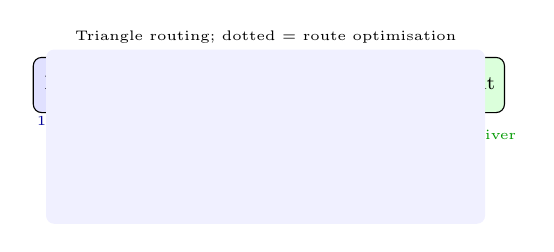
\begin{tikzpicture}[every node/.style={font=\scriptsize},scale=0.82]
\node[draw,fill=blue!12,rounded corners=3pt,minimum width=1.8cm,minimum height=0.7cm] (ha) at (0,1.6) {Home Agent};
\node[draw,fill=green!14,rounded corners=3pt,minimum width=1.8cm,minimum height=0.7cm] (fa) at (5,1.6) {Foreign Agent};
\node[draw,circle,fill=orange!18,minimum size=7mm] (mn) at (5,0) {MN};
\node[draw,circle,fill=violet!12,minimum size=7mm] (cn) at (0,0) {CN};
\draw[->,thick,blue!60!black] (cn) -- (ha) node[midway,above,font=\tiny] {1. to home addr};
\draw[->,thick,red!70!black] (ha) -- (fa) node[midway,above,font=\tiny] {2. tunnel to CoA};
\draw[->,thick,green!60!black] (fa) -- (mn) node[midway,right,font=\tiny] {3. deliver};
\draw[->,dashed,orange!70!black] (mn) -- (cn) node[midway,below,font=\tiny] {4. direct reply (optimised)};
\fill[blue!6,rounded corners=3pt] (-0.9,-0.55) rectangle (5.9,2.15);
\node[font=\tiny,fill=white,inner sep=1pt] at (2.5,2.35) {Triangle routing; dotted = route optimisation};
\end{tikzpicture}
\caption{Mobile IP: correspondent (CN) sends to home address; home agent tunnels to foreign agent / care-of address; MN can reply directly when optimised.}
\label{fig:mobile-ip}
\end{figure}

\textbf{Cellular evolution:} 2G (GSM, digital voice), 3G (UMTS, Mbps data), 4G LTE (all-IP, OFDMA, 100\,Mbps, EPC core with MME/S-GW/P-GW, eNodeB base stations), 5G (mmWave + sub-6\,GHz, massive MIMO, beamforming, network slicing, ultra-low latency via edge, gNodeB and service-based core). In all generations a base station covers a cell; handoff is network-controlled and make-before-break to keep calls alive.

\section{Throughput, Fairness, and Why Wi-Fi Feels Slower}\label{sec:throughput}
Raw rate is not goodput. Each frame pays DIFS + backoff + preamble + header + SIFS + ACK. At 54\,Mbps, a 1500\,B frame takes $222\,\mu$s on air but $\approx 50+67+222+10+30\approx 379\,\mu$s with overhead, so single-station goodput $\approx 31.6$\,Mbps (58\%). With $n$ contending stations, collisions and larger CW further reduce it.

Example: two stations saturated, CW$_{\min}=15$. Average backoff $\approx 7.5$ slots $=67\,\mu$s. Collision probability $p\approx 1/(1+\mathrm{CW})\approx 6\%$ with two stations; on collision CW doubles and retries add delay. Aggregate goodput drops to 20--25\,Mbps. Capture effect and rate heterogeneity worsen fairness: a slow 6\,Mbps station occupying air 9$\times$ longer than a 54\,Mbps station drags everyone (performance anomaly); 802.11e TXOP and airtime fairness mitigate by granting equal airtime, not equal packets.

Power and scanning cost matter for phones: passive scanning across 11 channels at 100\,ms per channel costs $>1$\,s to discover APs; active probing cuts this to tens of ms but burns energy. Hence phones prefer to stay associated and use 802.11k/v neighbour reports to prune scan lists.

\subsection{Worked Example: Goodput in Numbers}
Take 802.11g at 54\,Mbps, slot $9\,\mu$s, DIFS $28\,\mu$s, SIFS $10\,\mu$s, preamble $20\,\mu$s, ACK $14$\,B at 24\,Mbps $\approx 30\,\mu$s. For a 1500\,B payload:
\begin{itemize}[itemsep=0.25em]
    \item Data airtime: $(1500\times8)/54\text{Mbps}\approx 222\,\mu$s plus preamble $20\,\mu$s $=242\,\mu$s.
    \item Overhead before data: DIFS $28\,\mu$s + average backoff $7.5\times9=67.5\,\mu$s.
    \item Overhead after data: SIFS $10\,\mu$s + ACK $30\,\mu$s.
    \item Total per frame $\approx 28+67.5+242+10+30=377.5\,\mu$s, goodput $\approx 1500\times8/377.5\,\mu\text{s}\approx 31.8$\,Mbps.
\end{itemize}
With three saturated stations collision rate rises; simulation with CW doubling shows aggregate goodput falls to $\approx 22$\,Mbps, so per-station share is $\approx 7$\,Mbps despite 54\,Mbps PHY rate.

\section{Wireless Security Glimpse: WEP \texorpdfstring{$\to$}{to} WPA2/3}\label{sec:wireless-sec}
WEP (Wired Equivalent Privacy) failed because it reused RC4 keystreams with a 24-bit IV: after $\approx 5000$ packets an IV repeats, and with enough repeats the keystream is recovered; plus CRC32 is not a MAC, so bit-flipping goes undetected. WPA2 fixes both: AES-CCMP provides confidentiality and integrity with a 48-bit packet number (PN) that never repeats within a key lifetime, and 802.1X/EAP does mutual authentication via a 4-way handshake deriving a fresh PTK per session. WPA3 adds forward secrecy (SAE handshake) and opportunistic encryption. Details of crypto, MACs and handshakes are in Ch.~\ref{ch:security}.

\section{Chapter Notes}
802.11 standards are IEEE 802.11a/b/g/n/ac/ax (Wi-Fi 4/5/6); cellular specs are 3GPP LTE/NR. Tanenbaum \& Wetherall and Kurose \& Ross cover wireless chapters with matching figures; the hidden/exposed duality and NAV are the exam favourites. Next chapter builds the crypto that makes WPA2/3 and TLS possible.

\section{Exercises}\label{sec:ch07-exercises}
\begin{enumerate}[label=E7.\arabic*, leftmargin=*, itemsep=0.8em]
    \item \textbf{Hidden vs.\ exposed.} Draw $A$--$B$--$C$--$D$ line topology with ranges $A\leftrightarrow B$, $B\leftrightarrow A,C$, $C\leftrightarrow B,D$, $D\leftrightarrow C$. Identify hidden and exposed pairs and state for each whether RTS/CTS helps, hurts, or is neutral; quantify overhead if RTS/CTS $=20$\,B and data $=1500$\,B at 54\,Mbps.
    \item \textbf{CSMA/CA walk-through.} Two stations both wait DIFS and pick backoff 2 and 5 (CW=7, slot 9\,$\mu$s). Tabulate countdown slot by slot including freeze when the first transmits, compute total idle time before the second starts, and show CW evolution if the second collides twice then succeeds.
    \item \textbf{Channel planning.} In 2.4\,GHz with channels 1/6/11, place 4 APs on a floor to minimise co-channel interference. Explain why 5\,GHz with 24 non-overlapping 20\,MHz channels changes the plan, and compute max aggregate throughput if each AP does 150\,Mbps.
    \item \textbf{Rate vs.\ range.} Using the SNR thresholds in the listing, a station moves from SNR 28\,dB to 12\,dB. What rate is chosen before/after? If BER at 64-QAM is $10^{-3}$ at 12\,dB but $10^{-5}$ at BPSK, estimate retransmissions per 1000 frames and effective goodput.
    \item \textbf{Mobile IP triangle.} CN sends 10 packets to MN's home address while MN is away. Trace each packet's path with and without route optimisation, count hops and tunnel overhead, and explain why ingress filtering can break naive direct replies from MN.
\end{enumerate}
% End of Chapter 7
